% !TEX root=/home/tavant/these/manuscript/src/manuscript.tex

% \FloatBarrier

    
    \section{Electron temperature saturation in experiments}
    
    
    In \citet{raitses2006}, the authors compare the maximum of the axial profile of the electron temperature $\hat{\Te}$ measured in a \ac{HET} with two different wall materials, one with a very low emissivity (carbon velvet material), the other the conventional \ac{BN} ceramic.
    \Cref{fig-raiteses2006} reproduces the results obtained in \citet{raitses2006}.

    \begin{figure}[hbt]
      \centering
      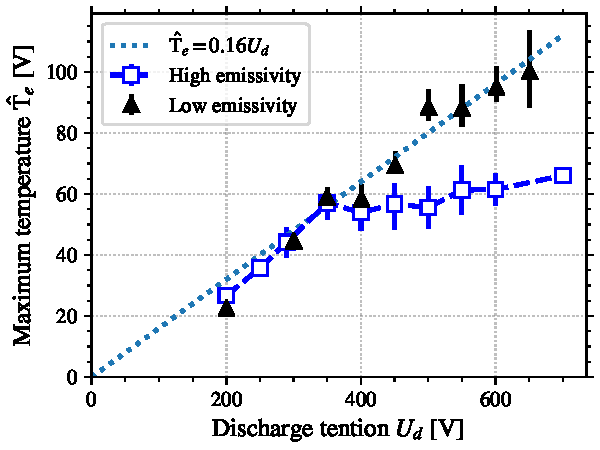
\includegraphics[width=\defaultwidth]{Raiteses_remaked.pdf}
      \caption{ The dependence of the maximum electron temperature on the discharge  voltage for a conventional thruster with high-SEE \acs{BN} channel walls and the segmented thruster with low-SEE floating segmented electrodes made of carbon velvet material. Reproducibility of measurements is shown by error bars. Adapted from \citet[Fig. 3]{raitses2006} }
      \label{fig-raiteses2006}
    \end{figure}

    They observed that with the \ac{BN} ceramic, the values of $\hat{\Te}$ present a maximum value that cannot be exceeded, while the results with the low emissivity material do not present such maximum.
    The maximum value of $\hat{\Te}$ measured for \ac{BN} ceramic is $\hat{\Te}^1 = 55 \pm 6\,\volt$, the error corresponds to reproducibility of the measurements (manually extracted from \citep[Fig. 3]{raitses2006}, reproduced in \cref{fig-raiteses2006}).
    
    The saturation of the temperature is expected to be due to the \ac{SCL} regime, which increase the electron power losses.
    For a \ac{BN} wall, we have $\crover\simeq 35\,\volt$ \citep{smirnov2004}.
    The value of $\Te^1$ observed experimentally,  $\hat{\Te}^1$, is higher than the value observed in the \ac{PIC} simulations and obtained with the sheath model, which close to $\Te^1 = 45\,\volt$.
    however, the agreement is significantly better than with the isothermal sheath model prediction 
    \begin{equation} \label{eq-Temaxisothermal}
      \Te^1_{\rm , isothermal} \simeq \frac{\crover}{2} \simeq 17.5 \,\volt.
    \end{equation}
    
    One possible explanation of the difference is the anisotropy of the electrons.
    Indeed, the probe measurements measure the average electron temperature, in contrast with the sheath theory which suppose that the electrons are isotropic.
    